\documentclass[sigconf,nonacm]{acmart}

\AtBeginDocument{%
  \providecommand\BibTeX{{Bib\TeX}}}

\settopmatter{printacmref=false, printfolios=true}
\setcopyright{none}
\copyrightyear{2026}
\acmYear{2026}
\acmDOI{}
\acmConference[OWiSR 2026]{Research Project Report}{June 2026}{Poland}
\acmISBN{}

\usepackage{booktabs}
\usepackage{tabularx}
\usepackage{array}

\graphicspath{{../../assets/}{figures/}}

\title{Adapting DiffDIS to a DiT-Based Diffusion Backbone for Dichotomous Image Segmentation}

\author{Jakub Wilk}
\affiliation{%
  \institution{Gdansk University of Technology}
  \city{Gdansk}
  \country{Poland}}

\author{Kacper Sochacki}
\affiliation{%
  \institution{Gdansk University of Technology}
  \city{Gdansk}
  \country{Poland}}

\author{Jakub Grunwald}
\affiliation{%
  \institution{Gdansk University of Technology}
  \city{Gdansk}
  \country{Poland}}

\renewcommand{\shortauthors}{Wilk, Sochacki, and Grunwald}

\begin{abstract}
Dichotomous image segmentation (DIS) requires category-agnostic binary masks with accurate object boundaries and fine internal structure. DiffDIS showed that a pre-trained latent diffusion model can be repurposed for this task by combining VAE-space mask generation, one-step denoising, auxiliary edge prediction, and mask-edge interaction. In this work we document our reproduction of DiffDIS and an architectural modification that replaces the original U-Net denoising backbone with a DiT-style UniDiffuser transformer. The modified model adapts the image-latent input projection to an eight-channel segmentation input, uses Vision Transformer features as image conditioning, injects mutual cross-domain attention between mask and edge streams, and fine-tunes the VAE decoder with a reconstruction loss. We evaluate the reproduced baseline and the modified model on the original DIS5K validation/test splits and on a ThinObject5K benchmark. The reproduction obtains strong results close to the expected DiffDIS behavior, while the transformer-based modification substantially underperforms on the original benchmark. Rather than presenting the modification as an improvement, this report analyzes it as a controlled engineering study: it identifies which parts of the DiffDIS design were transferable, which assumptions became fragile under a DiT backbone, and what would be required to stabilize future transformer-based dense prediction variants.
\end{abstract}

\begin{CCSXML}
<ccs2012>
 <concept>
  <concept_id>10010147.10010257.10010293.10010319</concept_id>
  <concept_desc>Computing methodologies~Image segmentation</concept_desc>
  <concept_significance>500</concept_significance>
 </concept>
 <concept>
  <concept_id>10010147.10010257.10010293.10010294</concept_id>
  <concept_desc>Computing methodologies~Neural networks</concept_desc>
  <concept_significance>300</concept_significance>
 </concept>
</ccs2012>
\end{CCSXML}

\ccsdesc[500]{Computing methodologies~Image segmentation}
\ccsdesc[300]{Computing methodologies~Neural networks}

\keywords{dichotomous image segmentation, diffusion models, DiffDIS, DiT, UniDiffuser, Vision Transformer}

\begin{document}
\maketitle

\section{Introduction}
Dichotomous image segmentation (DIS) is the task of producing a high-accuracy binary foreground mask for arbitrary objects in natural images. In contrast to class-specific semantic segmentation, DIS is category agnostic. Unlike coarse salient object detection, it emphasizes accurate object silhouettes, thin structures, holes, and high-frequency details. This makes the task difficult: a successful model needs a wide receptive field to understand global object extent, but it must also preserve local detail at boundaries and internal structures.

DiffDIS addresses this problem by repurposing the capacity of pre-trained latent diffusion models for segmentation \cite{yu2025diffdis}. The original method maps RGB images, masks, and edge maps into the VAE latent space, trains a denoising model to recover mask and edge latents in a single step, and uses an auxiliary edge task to make the generative process more deterministic. This design is attractive for a student research project because it combines modern diffusion models with a concrete, measurable dense prediction task.

Our work had two goals. First, we reproduced the DiffDIS training and evaluation pipeline on the DIS5K benchmark \cite{qin2022dis}. Second, we implemented a more experimental modification: replacing the U-Net-style denoising backbone used by DiffDIS with a transformer-based diffusion backbone inspired by DiT \cite{peebles2023dit} and implemented through UniDiffuser \cite{bao2023unidiffuser}. The motivation was to test whether the mask-edge formulation of DiffDIS can be transferred to a transformer denoiser while preserving the one-step segmentation pipeline.

The resulting system is not a performance improvement over the reproduced baseline. On the original DIS5K splits, the modified model is substantially worse across MAE, maxF, structural similarity, IoU, and HCE. Nevertheless, the experiment is useful because it exposes the sensitivity of diffusion-based segmentation to the denoising backbone, conditioning pathway, and loss placement. The main contribution of this report is therefore a documented negative result with implementation details, reproducible metrics, and an analysis of likely failure modes.

Our code is available at:
\begin{center}
\url{https://github.com/PyroX2/DiffDIS/tree/dit}
\end{center}

\section{Background}
\subsection{Dichotomous Image Segmentation}
DIS was introduced to study highly accurate binary segmentation of category-agnostic objects \cite{qin2022dis}. The DIS5K dataset contains high-resolution images with fine annotations and is split into training, validation, and multiple test subsets with increasing structural complexity. The task is usually evaluated with region, structure, and boundary-sensitive metrics, including MAE, F-measure, weighted F-measure, S-measure, E-measure, IoU, Dice, accuracy, BER, and HCE. In our experiments we report the same family of metrics computed by the evaluation utilities included in the DiffDIS codebase.

\subsection{Diffusion Models for Dense Prediction}
Denoising diffusion probabilistic models learn to reverse a gradual noising process \cite{ho2020ddpm}. Latent diffusion models reduce the computational cost by operating in the latent space of an autoencoder rather than directly on pixels \cite{rombach2022latent}. This idea has been reused in several dense prediction systems, including depth estimation and segmentation-like tasks, because the pre-trained generative representation often encodes both global scene layout and local detail \cite{ke2024marigold}.

DiffDIS adapts this principle to segmentation. Instead of sampling an image through many denoising steps, it trains the network at the final timestep and performs one-step prediction, following the broader move toward efficient distilled diffusion models such as SD-Turbo \cite{sauer2023sdturbo}. The method also predicts mask and edge targets together. The edge task supplies boundary information and reduces the mismatch between stochastic generation and deterministic segmentation.

\subsection{Transformer Diffusion Backbones}
Classic latent diffusion systems typically use U-Net denoisers. DiT showed that transformer blocks can also serve as scalable denoising backbones over latent patches \cite{peebles2023dit}. UniDiffuser extends this direction to a unified multi-modal diffusion framework using a transformer parameterization \cite{bao2023unidiffuser}. This makes UniDiffuser an appealing candidate for experimentation: it already exposes image and text embedding interfaces and uses transformer blocks that can be modified with attention-based interactions.

However, replacing a U-Net with a transformer is not a drop-in change for segmentation. U-Nets naturally preserve multi-scale spatial structure through encoder-decoder skip connections, while transformer backbones depend heavily on tokenization, embedding dimensions, and conditioning design. Our modification therefore tests not only whether DiT can denoise segmentation latents, but also whether DiffDIS-style mask-edge conditioning survives a different inductive bias.

\section{Baseline Method}
The reproduced baseline follows the public DiffDIS repository and the paper's overall design. Given an RGB image, ground-truth mask, and generated edge map, the VAE encoder maps all three images into latent space. RGB latents are used as a condition, while mask and edge latents are concatenated along the batch dimension and noised at timestep $T=999$. The denoising model receives the noisy target latent together with the image condition and predicts the noise needed to recover a clean mask or edge latent.

Two details are central. First, mask and edge are distinguished by Batch-Discriminative Embedding (BDE), a compact task label encoding also used in diffusion-based geometry systems \cite{fu2024geowizard}. Second, the model uses an interaction module between mask and edge features, so the auxiliary edge task can directly inform mask prediction. This is the mechanism that motivates our own mutual cross-domain attention layer in the transformer version.

The baseline uses CutMix augmentation \cite{yun2019cutmix}, latent-space training, and one-step denoising. In our reproduction we evaluated the model on the original DIS5K validation and test subsets and on a ThinObject5K benchmark. These reproduced results are used as the empirical reference point for the modified model.

\section{Proposed Modification}
\subsection{Replacing the Denoising Backbone}
The core modification is in \texttt{run\_train.py}: the original DiffDIS U-Net denoiser is replaced with \texttt{UniDiffuserModel} loaded from \texttt{thu-ml/unidiffuser-v1}. Because the DiffDIS-style input concatenates RGB latents with noisy target latents, the UniDiffuser image input projection must accept eight channels instead of four. We implement this in \texttt{replace\_dit\_in\_dim}: the original projection weights are duplicated across the channel dimension and scaled by $0.5$, giving the model a symmetric initialization for the RGB and target halves of the input.

This is a conservative initialization: it avoids randomizing the first projection completely, but it also assumes that the pre-trained projection can be meaningfully reused for the new channel layout. This approach is the same as the one presented in the original DiffDIS paper.

\subsection{Vision Transformer Conditioning}
The original DiffDIS model uses text-related conditioning infrastructure with an empty prompt and image latents. Our modified implementation introduces a frozen ViT-B/16 image-feature extractor \cite{dosovitskiy2021vit}. In the code, this corresponds to the Hugging Face checkpoint \path{google/vit-base-patch16-224}. The ViT hidden states are projected to match the expected conditioning dimension and duplicated for the mask and edge streams. This produces image-aware prompt embeddings for the UniDiffuser forward pass.

Only the projection layer is intended to adapt the ViT representation to the segmentation denoiser. The ViT itself is kept frozen. This keeps the number of trainable parameters lower and avoids overfitting the image classifier backbone on a relatively small segmentation dataset, but it may also limit the model's ability to learn fine-grained boundary cues.

\subsection{Mutual Cross-Domain Attention}
We added \texttt{mutual\_cross\_domain\_attention.py}, implementing a direct interaction between mask tokens and edge tokens. The batch is structured so that the first half corresponds to mask samples and the second half to edge samples. The module projects both domains to queries, keys, and values, then performs two attention operations:
\begin{equation}
  \mathrm{Attn}_{m \leftarrow e} = \mathrm{softmax}\left(\frac{Q_m K_e^\top}{\sqrt{d}}\right)V_e,
\end{equation}
\begin{equation}
  \mathrm{Attn}_{e \leftarrow m} = \mathrm{softmax}\left(\frac{Q_e K_m^\top}{\sqrt{d}}\right)V_m.
\end{equation}
The outputs are concatenated back along the batch dimension and projected to the original embedding dimension.

In \texttt{run\_train.py}, this module is wrapped around the middle transformer block through \texttt{DBIATransformerBlockWrapper}. The wrapper runs the original transformer block, normalizes its output, applies mutual cross-domain attention, and adds the result residually. This mirrors the spirit of DiffDIS's Detail-Balancing Interactive Attention, but in a transformer-token setting instead of a U-Net feature-map setting.

\subsection{VAE Decoder Fine-Tuning}
The modified training freezes the VAE encoder and quantization convolution, while allowing the decoder and post-quantization convolution to update. The generator objective predicts noise for mask and edge latents:
\begin{equation}
  \mathcal{L}_{gen} =
  \left\|\epsilon_{\theta}^{mask} - \epsilon^{mask}\right\|_2^2 +
  \left\|\epsilon_{\theta}^{edge} - \epsilon^{edge}\right\|_2^2 .
\end{equation}
After one denoising step, the predicted mask latent is decoded and compared with the ground-truth mask image:
\begin{equation}
  \mathcal{L}_{vae} =
  \left\|D_{\phi}(\hat{z}_{mask}) - y_{mask}\right\|_2^2 .
\end{equation}
The VAE decoder has its own Adam optimizer and learning rate. This was intended to adapt the decoder to binary mask reconstruction, but it introduces a second moving component into training. If the denoiser and decoder drift at different speeds, the latent objective and pixel reconstruction objective can become poorly aligned.

\subsection{Architecture Overview}
Figure~\ref{fig:proposed-architecture} summarizes the final modified architecture. The RGB image is encoded by a frozen ViT and used as conditioning for both paths. The mask-generation and edge-detection paths share the same UniDiffuser transformer core, receive the eight-channel concatenation of RGB and noisy target latents, and exchange information through the mutual cross-domain attention wrapper in the middle transformer block. The two paths predict mask and edge noise separately and are supervised with MSE losses.

\begin{figure*}[!t]
  \centering
  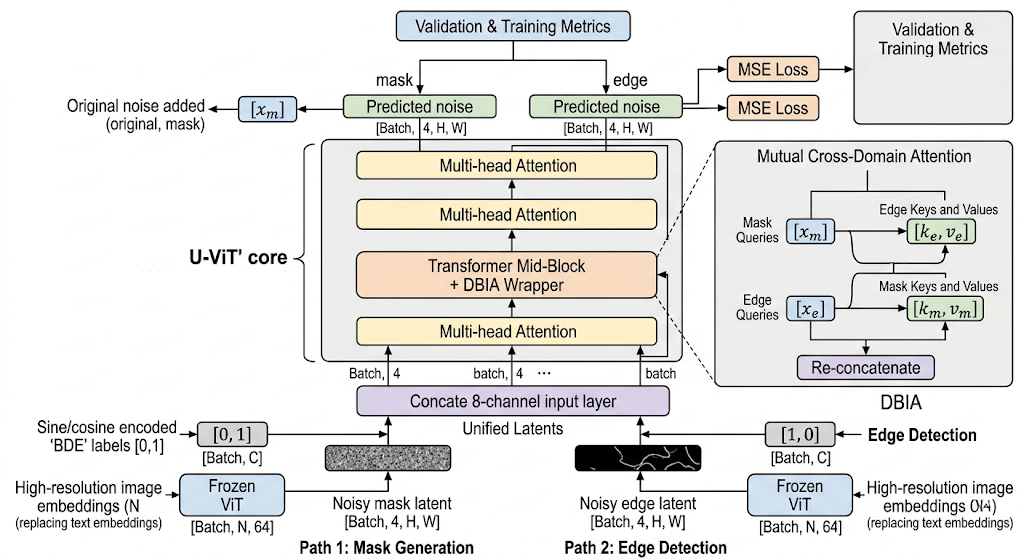
\includegraphics[width=0.92\textwidth]{proposed_architecture.png}
  \caption{Architecture of the modified DiffDIS model. The original U-Net denoiser is replaced with a UniDiffuser-style transformer core, while ViT image embeddings, BDE labels, mask/edge latent paths, and mutual cross-domain attention provide task conditioning and mask-edge interaction.}
  \Description{Diagram of the proposed architecture with two paths for mask generation and edge detection. Frozen ViT embeddings condition both paths, noisy mask and edge latents enter an eight-channel input layer, a U-ViT core contains a DBIA wrapper, and the model predicts separate mask and edge noise supervised by MSE losses.}
  \label{fig:proposed-architecture}
\end{figure*}

\section{Implementation}
The implementation is based on the DiffDIS codebase and the Hugging Face \texttt{diffusers} library \cite{diffusers2024}. The main modified files are:
\begin{itemize}
  \item \texttt{run\_train.py}: UniDiffuser loading, input projection replacement, ViT conditioning, VAE decoder training, logging, checkpointing, and validation call.
  \item \texttt{mutual\_cross\_domain\_attention.py}: mask-edge attention module.
  \item \texttt{val\_utils.py}: validation loop and metric logging.
  \item \texttt{scripts/run\_train.sh}: training configuration for the modified run.
  \item \texttt{utils/config.py}, \texttt{test\_score.py}, and \texttt{get\_contour.py}: local dataset and evaluation paths.
\end{itemize}

The modified training configuration uses batch size 2 and image size 512. The model is trained with Adam, a generator learning rate of $10^{-4}$, and a separate VAE decoder learning rate of $10^{-4}$. RGB, mask, and edge images are encoded by the VAE. Mask and edge latents are noised at timestep 999 and are predicted jointly. Validation is run on DIS-VD during training, and final evaluation is performed with the same metric utilities for the original and modified models.

\begin{figure}[t]
  \centering
  \includegraphics[width=\linewidth]{pipeline.png}
  \caption{Original DiffDIS pipeline from the project assets. Our modification keeps the latent mask/edge formulation and one-step denoising objective, but replaces the U-Net denoising backbone with a UniDiffuser transformer and adds ViT-based image conditioning.}
  \Description{A pipeline diagram showing RGB, mask, and edge inputs encoded into latent space and processed by a diffusion denoising model.}
  \label{fig:pipeline}
\end{figure}

\section{Experimental Setup}
\subsection{Datasets}
We report two evaluation settings. The first is the original DIS5K setting, including DIS-VD and DIS-TE1 through DIS-TE4. The second is a ThinObject5K benchmark, marked as ``New dataset'' in our result sheets, with DIS-VD and DIS-TE1 measurements. This benchmark uses ThinObject5K for training and COIFT+HRSOD for validation, and its validation/test settings are reported as DIS-VD and DIS-TE1, respectively, with the standard ThinObject5K train/test split used for testing. The ThinObject5K combination is useful as a secondary sanity check, but it should not be interpreted as a replacement for the full DIS5K benchmark.

\subsection{Metrics}
The result sheets include MAE, BER, maximum F-measure (maxF), average F-measure (avgF), weighted F-measure (wFm), S-measure (Sm), adaptive E-measure (adpEm), mean Dice, mean IoU, accuracy, and HCE. Lower is better for MAE, BER, and HCE; higher is better for the remaining metrics. To keep the paper readable, the main tables report MAE, maxF, Sm, mean IoU, and HCE. These cover pixel error, region quality, structural similarity, overlap, and correction effort.

\subsection{Compared Models}
We compare two models:
\begin{description}
  \item[Reproduced DiffDIS:] our reproduction of the original project pipeline, used as the baseline.
  \item[Modified DiT model:] our UniDiffuser/ViT/mutual-attention variant implemented on the \texttt{dit} branch.
\end{description}
The comparison therefore measures the effect of our architectural modification rather than a broad benchmark against all published DIS methods.

\section{Results}
Table~\ref{tab:original-results} shows results on the original DIS5K validation and test subsets. The reproduced baseline is consistently strong, with average MAE $0.0294$, average maxF $0.9048$, average Sm $0.9026$, and average mean IoU $0.8388$. The modified DiT model is much weaker, with average MAE $0.4117$, average maxF $0.3106$, average Sm $0.4084$, and average mean IoU $0.2487$.

\begin{table*}[t]
\centering
\caption{Results on the original DIS5K validation/test setting. MAE and HCE are lower-is-better; maxF, Sm, and mIoU are higher-is-better.}
\label{tab:original-results}
\begin{tabular}{lrrrrrrrrrr}
\toprule
& \multicolumn{5}{c}{Reproduced DiffDIS} & \multicolumn{5}{c}{Modified DiT model} \\
\cmidrule(lr){2-6}\cmidrule(lr){7-11}
Dataset & MAE & maxF & Sm & mIoU & HCE & MAE & maxF & Sm & mIoU & HCE \\
\midrule
DIS-VD  & 0.0294 & 0.9005 & 0.9006 & 0.8341 & 1061 & 0.4156 & 0.3122 & 0.4041 & 0.2502 & 1443 \\
DIS-TE1 & 0.0312 & 0.8785 & 0.8890 & 0.8133 & 100  & 0.4461 & 0.2337 & 0.3666 & 0.1843 & 235 \\
DIS-TE2 & 0.0305 & 0.9068 & 0.9072 & 0.8423 & 267  & 0.4186 & 0.3083 & 0.4033 & 0.2454 & 491 \\
DIS-TE3 & 0.0238 & 0.9322 & 0.9202 & 0.8712 & 594  & 0.3958 & 0.3378 & 0.4276 & 0.2719 & 925 \\
DIS-TE4 & 0.0320 & 0.9058 & 0.8962 & 0.8333 & 2747 & 0.3825 & 0.3608 & 0.4405 & 0.2915 & 3433 \\
\midrule
Average & 0.0294 & 0.9048 & 0.9026 & 0.8388 & 953.8 & 0.4117 & 0.3106 & 0.4084 & 0.2487 & 1305.4 \\
\bottomrule
\end{tabular}
\end{table*}

The gap is too large to attribute to metric noise. On DIS-TE1, maxF decreases from $0.8785$ to $0.2337$ and mean IoU decreases from $0.8133$ to $0.1843$. Even on DIS-TE4, where the modified model obtains its highest maxF among the original test subsets, it remains far below the reproduced baseline.

Table~\ref{tab:new-results} reports the ThinObject5K benchmark. The modified model is still weaker, but the gap is less uniform. On the benchmark's DIS-VD subset, reproduced DiffDIS obtains maxF $0.7575$ and the modified model obtains $0.5457$. On the benchmark's DIS-TE1 subset, reproduced DiffDIS obtains maxF $0.9326$, while the modified model obtains $0.5217$. The result suggests that the modified model can learn some foreground structure, but not with the precision needed for DIS.

\begin{table}[t]
\centering
\caption{Results on the ThinObject5K benchmark.}
\label{tab:new-results}
\begin{tabular}{lrrrr}
\toprule
Model / Dataset & MAE & maxF & Sm & mIoU \\
\midrule
Reproduced, DIS-VD  & 0.0428 & 0.7575 & 0.8065 & 0.6594 \\
Modified, DIS-VD    & 0.1389 & 0.5457 & 0.6794 & 0.4689 \\
Reproduced, DIS-TE1 & 0.0276 & 0.9326 & 0.9105 & 0.8782 \\
Modified, DIS-TE1   & 0.2487 & 0.5217 & 0.5630 & 0.4174 \\
\bottomrule
\end{tabular}
\end{table}

Figure~\ref{fig:vae-comparison} gives a qualitative comparison of two internal training variants of the modified model. In both panels, the grids show reference binary masks together with model predictions. With the VAE kept frozen, the predictions are coarse and blurred, often preserving only a weak foreground location. Allowing the VAE decoder to train produces visibly sharper masks and better recovery of thin structures, although the predictions still remain less clean than the reproduced DiffDIS baseline. This supports the quantitative observation that the DiT-based variant can learn foreground structure but needs stronger stabilization before it can match the original U-Net-based pipeline.

\begin{figure}[!t]
  \centering
  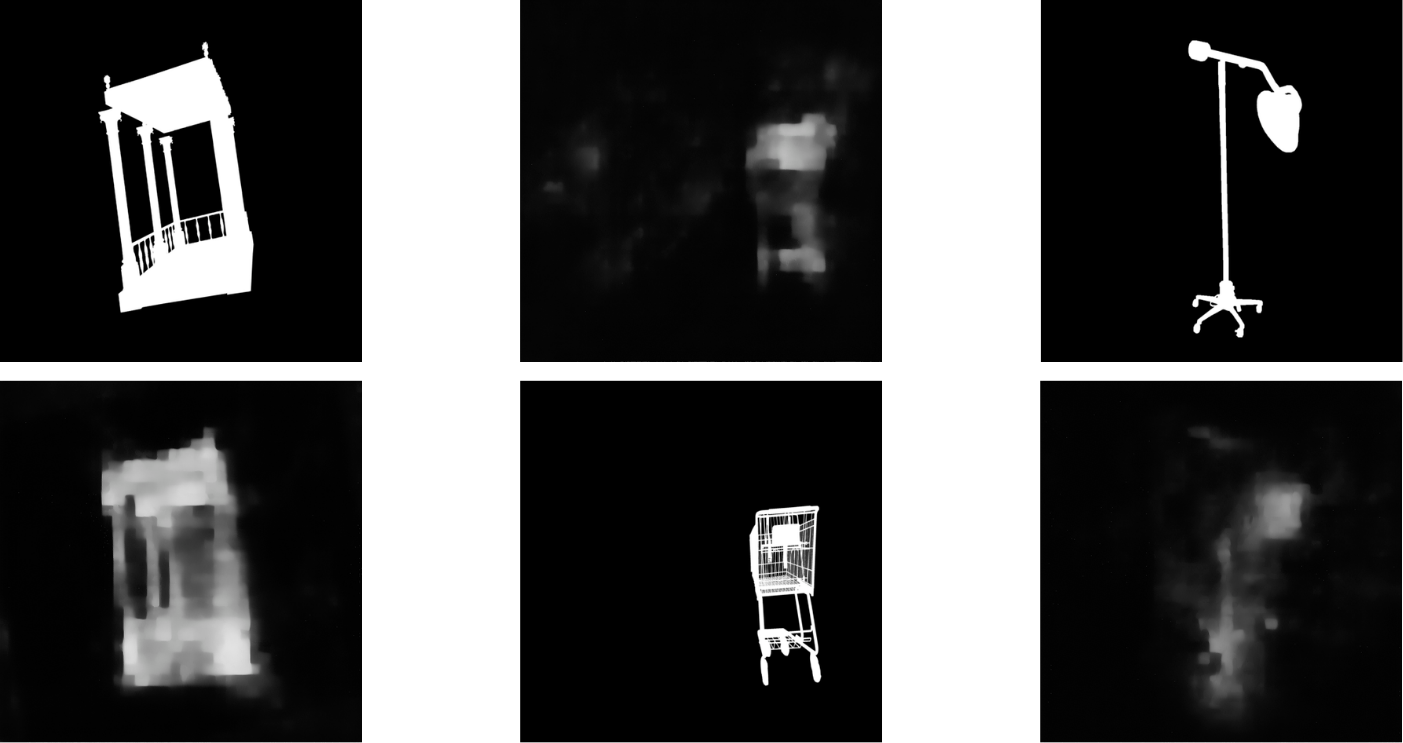
\includegraphics[width=\linewidth]{frozen_vae.png}

  \small (a) Frozen VAE.

  \vspace{0.5em}

  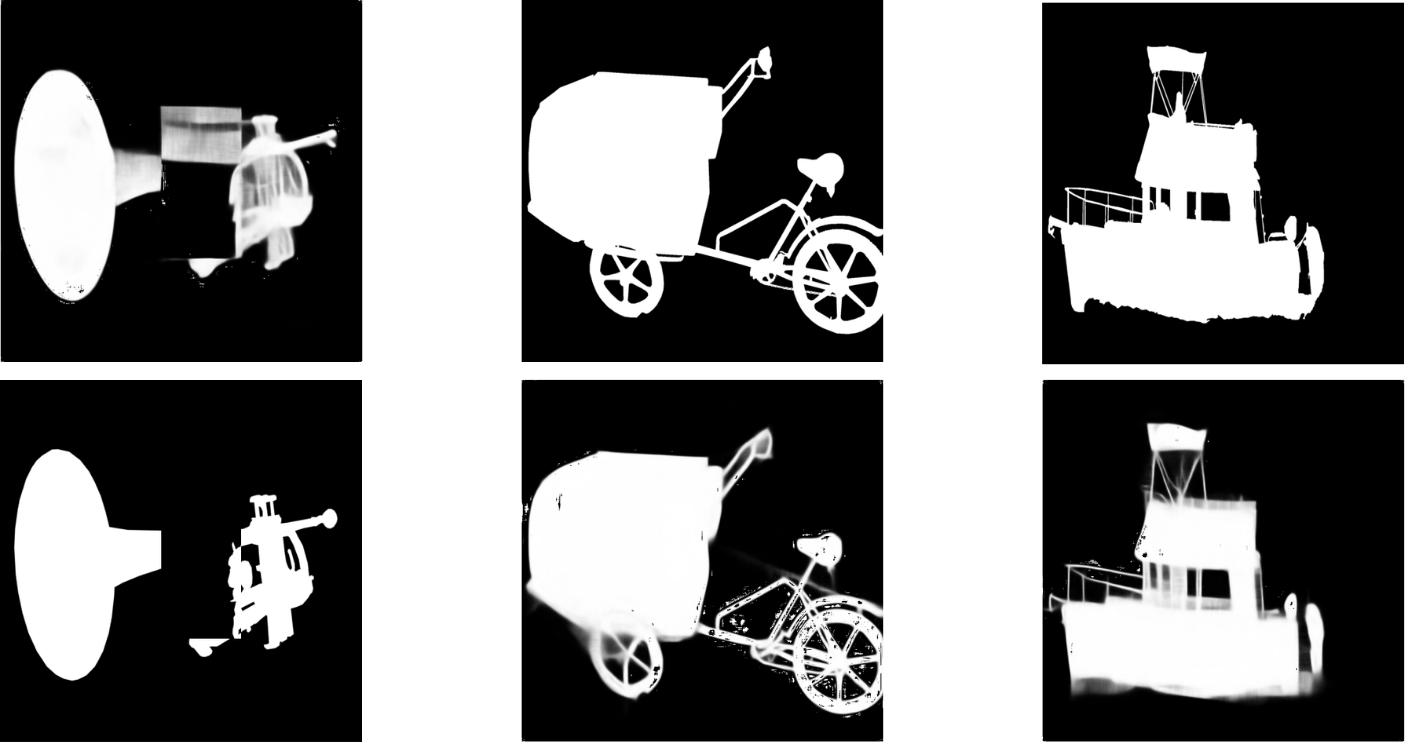
\includegraphics[width=\linewidth]{trained_vae.png}

  \small (b) Trainable VAE decoder.
  \caption{Qualitative comparison of two VAE training variants in the modified model. The frozen VAE variant produces diffuse foreground blobs, while training the VAE decoder improves object sharpness and boundary recovery.}
  \Description{Two side-by-side qualitative comparison grids showing frozen and trainable VAE variants. The frozen VAE predictions are blurrier; the trainable VAE decoder predictions are sharper.}
  \label{fig:vae-comparison}
\end{figure}

\section{Discussion}
\subsection{What Worked}
The reproduction results show that the evaluation pipeline, data preparation, edge generation, and metric computation are functional. The baseline numbers are coherent across DIS-VD and DIS-TE subsets: easier and harder subsets vary as expected, and the model maintains high mask quality across several metrics.

The modified model also validates some engineering assumptions. The UniDiffuser forward pass can be adapted to accept the eight-channel latent input. The batch arrangement for mask and edge streams works with transformer tokens, and the mutual attention module can be inserted into the middle transformer block without breaking shape compatibility. The validation code also successfully evaluates both the reproduced and modified outputs with the same metric suite.

\subsection{Why the Modified Model Underperformed}
The main failure is likely architectural rather than a single coding issue. DiffDIS relies on the spatial inductive bias of the U-Net denoiser, including multi-scale feature processing and structured feature-map interaction. UniDiffuser's transformer backbone represents latent information differently, and our adaptation only modifies the input projection and one middle block. This may be insufficient for preserving segmentation boundaries.

The conditioning pathway is another likely bottleneck. ViT classification features are useful for global image semantics, but DIS depends on dense localization. A frozen ViT trained for classification may discard exactly the fine boundary information needed for segmentation. The projection from ViT hidden states into UniDiffuser prompt embeddings may also be too weak to replace the original DiffDIS multi-scale conditional injection.

Finally, the training objective changed in an important way. The baseline supervises denoised latents directly, while the modified implementation predicts noise and separately updates the VAE decoder with a pixel reconstruction loss. This creates a more complex optimization problem. If the decoder changes while the denoiser is still learning a stable latent target, the model may chase a moving reconstruction space.

\subsection{Lessons for Future Work}
Future transformer-based DiffDIS variants should probably preserve dense conditioning more explicitly. Possible directions include adding ControlNet-style spatial adapters, using a segmentation-pretrained visual encoder instead of a classification ViT, applying cross-domain attention at multiple transformer depths, or freezing the VAE decoder until the denoiser becomes stable. A direct ablation study would also be necessary: UniDiffuser without ViT conditioning, UniDiffuser without mutual attention, frozen versus trainable VAE decoder, and noise prediction versus direct denoised-latent supervision.

\section{Limitations}
This report has several limitations. First, the comparison is between our reproduction and our modified implementation, not a full re-benchmark of all DIS methods. Second, the additional dataset contains only two measured subsets, so conclusions from it are weaker than conclusions from the full DIS5K evaluation. Third, we did not run a complete ablation study, so the exact contribution of each modification cannot be isolated. Fourth, the modified model may require longer training, different learning rates, or a more carefully initialized conditioning pathway. The current results should therefore be read as evidence that the direct adaptation is unstable, not as proof that transformer diffusion backbones are unsuitable for DIS.

\section{Conclusion}
We reproduced DiffDIS and implemented a transformer-based modification using UniDiffuser, ViT conditioning, mutual cross-domain attention, and VAE decoder fine-tuning. The reproduced baseline achieved strong results on DIS5K, while the modified model substantially underperformed. This negative result is still informative: it shows that DiffDIS's success depends not only on using diffusion, but also on the spatial and conditioning structure of the denoising backbone. A future DiT-based DIS model should include stronger dense conditioning, more careful latent supervision, and ablations before it can compete with the U-Net-based DiffDIS pipeline.

\begin{acks}
This work was prepared as part of the OWiSR course project at Gdansk University of Technology.
\end{acks}

\bibliographystyle{ACM-Reference-Format}
\bibliography{diffdis_dit_refs}

\end{document}
